\textbf{Pour cette première partie, aucune justification n'est demandée et une seule réponse est possible par question. Pour chaque question, reportez son numéro sur votre copie et indiquez votre réponse.}

Une réponse fausse ou l'absence de réponse n'enlève aucun point.

\subsubsection*{Question 1}
$5-\dfrac{3}{2}$ est égal à :

\textbf{a.} $1$ \hfill \textbf{b.} $\dfrac{7}{2}$ \hfill \textbf{c.} $4$ \hfill \textbf{d.} $-\dfrac{5}{2}$

\subsubsection*{Question 2}
$\left(2^3\right)^{-5}$ est égal à :

\textbf{a.} $2^{-2}$ \hfill \textbf{b.} $2^{-15}$ \hfill \textbf{c.} $6^{-5}$ \hfill \textbf{d.} $2^8$

\subsubsection*{Question 3}
Un téléphone coûte 990 euros. Le prix baisse de 20 \%.

Son nouveau prix est :

\textbf{a.} $990\times 0{,}2$ \hfill \textbf{b.} $990\times\left(1+\dfrac{20}{100}\right)$ \hfill \textbf{c.} $990\times\left(-\dfrac{20}{100}\right)$ \hfill \textbf{d.} $990\times 0{,}8$

\subsubsection*{Question 4}
On considère un dé truqué tel que la probabilité d'obtenir un 5 et celle d'obtenir un 6 sont chacune égales à 0,3.

On lance le dé. La probabilité d'obtenir un nombre supérieur ou égal à 5 est :

\textbf{a.} $\dfrac{2}{6}$ \hfill \textbf{b.} $\dfrac{1}{6}$ \hfill \textbf{c.} $0{,}6$ \hfill \textbf{d.} $0{,}3$

\subsubsection*{Question 5}
Les solutions de l'équation $(x-2)(2x+1)=0$ sont :

\textbf{a.} $2$ et $-\dfrac{1}{2}$ \hfill \textbf{b.} $-2$ et $1$ \hfill \textbf{c.} $2$ et $\dfrac{1}{2}$ \hfill \textbf{d.} $2$ et $-1$

\subsubsection*{Question 6}
Voici les notes obtenues dans une classe lors d'un contrôle en mathématiques.
\begin{center}
\begin{tabular}{|c|c|c|c|c|}
\hline
Note & 7 & 10 & 12 & 14\\
\hline
Nombre d'élèves & 5 & 7 & 8 & 10\\
\hline
\end{tabular}
\end{center}
La note médiane de ce contrôle est :

\textbf{a.} $12$ \hfill \textbf{b.} $11$ \hfill \textbf{c.} $11{,}37$ \hfill \textbf{d.} $7{,}5$

\subsubsection*{Question 7}
On donne ci-dessous la courbe représentative $\mathcal{C}_f$ d'une fonction $f$ définie sur l'intervalle $[-4;3]$.
\begin{center}
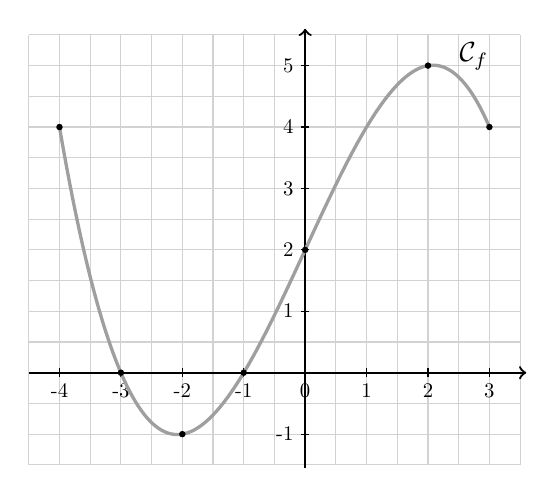
\begin{tikzpicture}[scale=0.78]
\draw[step=0.5,gray!35,thin] (-4.5,-1.5) grid (3.5,5.5);
\draw[->,thick] (-4.5,0)--(3.6,0);
\draw[->,thick] (0,-1.55)--(0,5.6);

\foreach \x in {-4,-3,-2,-1,0,1,2,3} {\draw (\x,0.07)--(\x,-0.07) node[below,scale=0.75] {\x};}
\foreach \y in {-1,1,2,3,4,5} {\draw (0.07,\y)--(-0.07,\y) node[left,scale=0.75] {\y};}

\begin{scope}
\clip (-4.5,-1.5) rectangle (3.5,5.5);

\draw[gray!75,very thick,domain=-4:3,samples=200,smooth] 
    plot (\x, {-1/6*pow(\x,3) + 13/6*\x + 2});
\end{scope}

\node at (2.75,5.15) {$\mathcal{C}_f$};


\fill (-4,4) circle (1.5pt);  
\fill (-3,0) circle (1.5pt);  
\fill (-2,-1) circle (1.5pt);  
\fill (-1,0) circle (1.5pt);  
\fill (0,2) circle (1.5pt);   
\fill (2,5) circle (1.5pt);   
\fill (3,4) circle (1.5pt);   
\end{tikzpicture}
\end{center}
L'ensemble des solutions de l'inéquation $f(x)\geqslant 0$ est :

\textbf{a.} $[0\,;\,3]$ \hfill \textbf{b.} $[-4\,;\,-2]$ \hfill \textbf{c.} $[-4\,;\,-3]\cup[-1\,;\,3]$ \hfill \textbf{d.} $[-4\,;\,-3]\cup[0\,;\,3]$

\subsubsection*{Question 8}
Dans le lycée Alpha, il y a 500 élèves.

150 lycéens pratiquent un sport.

Le pourcentage d'élèves pratiquant un sport dans ce lycée est égal à :

\textbf{a.} $15\ \%$ \hfill \textbf{b.} $35\ \%$ \hfill \textbf{c.} $30\ \%$ \hfill \textbf{d.} $65\ \%$




\begin{center}
\end{center}
